\chapter{Applications to Vapnik–Chervonenkis theory}

\section{Sets with Polynomial Discrimination}

The version of the Glivenko-Cantelli inequality we showed on chapter 2 can be generalized in multiple ways. First, we have to make some modifications in the proof of this theorem to make it work not just on intervals of the real line. The idea is to extend this property to a specific class of sets for which the final inequality will still be satisfied:

\begin{equation}
    \label{vc:1}
    \P\{\|P_n-P\| > \varepsilon\} \leq p(n) \cdot e^{-n \varepsilon^2 / 32}, \text{ for a polynomial } p(n).
\end{equation}

Remember from chapter 2 that:
\begin{itemize}
    \item $X_i$ is a i.i.d.~sample from a probability measure $P$.
    \item $P_n(A) = n^{-1}\sum \1_{X_i \in A} $ is the empirical measure given by $n$ sample points. 
    \item $\sigma_i$ is a Rademacher random variable.
\end{itemize}

In chapter 2 we assumed that $P$ is only defined on real intervals $(-\infty, t)$. Then, in the section maximal inequality, we strategically defined $(n+1)$ different disjoint intervals when ordering the sample
\[A_0 = (-\infty, X_{(1)}],\; A_1 = (X_{(1)}, X_{(2)}],\; \ldots,\; A_{n-1} = (X_{(n-1)}, X_{(n)}],\; A_n = (X_{(n)}, \infty].  \] % chktex 9
In each one of these intervals, we fixed a representative $t_j \in A_j$ so the function
\[ P_n^{\circ}(B) = n^{-1} \sum_{i = 1}^n \sigma_i \1_{X_i \in B}, \] 
reaches its supremum in one of the sets $B_k = (-\infty, t_k)$:
\[ \implies \exists k\leq n :\; \|P_n^\circ\| = |P_n^\circ(B_k)|.  \] 

Therefore, the $(n+1)$ term appears in the equation~\ref{gc:3}.

\vspace*{1em}

\subsection*{Quadrants in $\R^2$}

Now, imagine that instead of $(n+1)$ intervals we take ${(n+1)}^2$ quadrants in the form $(-\infty, a_i) \times (-\infty, b_j) \subseteq \R^2$:

\tikzmath{
    \a0 = -6.5; \a1 = -5; \a2 =-2; \a3 = 1; \a4 = 3.5; \a5 = 5;
    \b0 = -3; \b1 = -1.5; \b2 = 0.5; \b3 = 1.5; \b4 = 2.5; \b5 = 3.5;
 } 
\begin{tikzpicture}
    % Axis
    \draw[->] (-7, -4) -- (7, -4) node[right] {$x$};
    \draw[->] (-7, -4) -- (-7, 4) node[above] {$y$};
    % quadrant
    \draw [draw=black, fill=blue, opacity=0.3]
       (-7,\b4) -- (\a3,\b4) -- (\a3,-4) -- (-7,-4) -- cycle;
    \draw [draw=black, fill=red, opacity=0.3]
       (-7,\b3) -- (\a4,\b3) -- (\a4,-4) -- (-7,-4) -- cycle;
    \node[text=black] at (\a3,\b4) {$\bullet$};
    \node[text=black] at (\a3+0.6,\b4+0.3) {$(a_3,b_4)$};
    \node[text=black] at (\a4,\b3) {$\bullet$};
    \node[text=black] at (\a4+0.6,\b3+0.3) {$(a_4,b_3)$};
    \node[text=black] at (\a3,\b3) {$\bullet$};
    \node[text=black] at (\a3+0.6,\b3+0.3) {$(a_3,b_3)$};
    % Sample
    \coordinate (X1) at (-3,3); 
    \coordinate (X2) at (3,2); 
    \coordinate (X3) at (4,-2);
    \coordinate (X4) at (-1,-1);
    \coordinate (X5) at (-6,1);
    \node[text=black] at (X1) {$\overset{\bullet}{X_1}$};
    \node[text=black] at (X2) {$\overset{\bullet}{X_2}$};
    \node[text=black] at (X3) {$\overset{\bullet}{X_3}$};
    \node[text=black] at (X4) {$\overset{\bullet}{X_4}$};
    \node[text=black] at (X5) {$\overset{\bullet}{X_5}$};
    % vertical
    \draw [dashed] (\a0,-4) -- (\a0,4)  node[above] {$a_0$};
    \draw [dashed] (\a1,-4) -- (\a1,4)  node[above] {$a_1$};
    \draw [dashed] (\a2,-4) -- (\a2,4)  node[above] {$a_2$};
    \draw [dashed] (\a3,-4) -- (\a3,4)  node[above] {$a_3$};
    \draw [dashed] (\a4,-4) -- (\a4,4)  node[above] {$a_4$};
    \draw [dashed] (\a5,-4) -- (\a5,4)  node[above] {$a_5$};
    % horizontal
    \draw [dashed] (-7,\b0) -- (7,\b0)  node[right] {$b_0$};
    \draw [dashed] (-7,\b1) -- (7,\b1)  node[right] {$b_1$};
    \draw [dashed] (-7,\b2) -- (7,\b2)  node[right] {$b_2$};
    \draw [dashed] (-7,\b3) -- (7,\b3)  node[right] {$b_3$};
    \draw [dashed] (-7,\b4) -- (7,\b4)  node[right] {$b_4$};
    \draw [dashed] (-7,\b5) -- (7,\b5)  node[right] {$b_5$}; 
\end{tikzpicture}

\vspace*{1em}

Let $A_{i,j} = (-\infty, a_i) \times (-\infty, b_j)$ be the quadrants described previously. In this example, we choose $a_i$ and $b_i$ in such way that the $a_i$'s separate the sample horizontally and $b_j$ vertically (similar to how we did with the $t_j$'s in the 1-D case). Now, let $\AA_n = {\{A_{i,j}\}}_{i,j \leq n}$, and let $\AA$ be the collection of all quadrants in $\R^2$. We will see that even though $\AA_n \subset \AA$ is finite, it contains all of the information of $P_n^\circ$.

\vspace*{1em}

Let $X^i_j$ be the $i$-th coordinate of the point $X_j$, the formula for $P_n^\circ$ at a point $(x,y) \in \R^2$ is:

\[ P_n^\circ(x,y) = P_n^\circ((-\infty, x)\times(-\infty, y)) = n^{-1} \sum_{k = 1}^{n} \sigma_i \1_{X_k^1 < x}\cdot \1_{X_k^2 < y} \] 

Then, because of the way we chose $a_i$ and $b_j$, there exists $i, j$ such that $x \in (a_{i-1}, a_i)$ and $y \in (b_{j-1}, b_j)$. Thus,
\[ \forall k \leq n:\; \begin{array}{c}
    \1_{X_k^1 < x} = \1_{X_k^1 < a_i}\\
    \1_{X_k^2 < y} = \1_{X_k^2 < b_j}
\end{array} .\] 
It follows that all the relevant information of $\AA$ is contained in $\AA_n$ since $P_n^\circ(x,y) = P_n^\circ(a_{i},b_{j}) = P_n(A_{i,j})$ for some $i,j \in\N$. Thus, there exist $k_1, k_2\in \N$ such that
\[ \|P_n^\circ\|_\AA = \max_{A \in \AA_n}|P_n^\circ(A)| =  |P_n(A_{k_1,k_2})|. \]
Hence, 
\begin{equation} \label{vc:2}
    \everymath{\displaystyle}\arraycolsep=1.4pt\def\arraystretch{1.5}
    \begin{array}{rcl}
    \P\{ \|P_n^\circ\|_\AA > \tfrac{1}{4} \varepsilon \;|\; X \} & \leq & \sum_{i,j \leq n}\P\{ |P_n^\circ(A_{i,j})| > \tfrac{1}{4} \varepsilon \;|\; X \}\\
    & \leq & {(n+1)}^2 \cdot \P\{ |P_n^\circ(A_{k_1,k_2})| > \tfrac{1}{4} \varepsilon \;|\; X \} .
  \end{array}
\end{equation}
The rest of the steps in the proof of the Glivenko-Cantelli \text{theorem}~(\ref{glivenko-cantelli}) never depended on the fact that we used intervals (we will elaborate further in the next section). Therefore, the formula~\ref{vc:1}, should be changed to:

\begin{equation}
    \label{vc:3}
    \P\{\|P_n-P\|_{\AA} > \varepsilon\} \leq {(n+1)}^2 \cdot e^{-n \varepsilon^2 / 32}
\end{equation}

\[ \implies \P\{\|P_n-P\|_\AA > \varepsilon\} \overset{p}{\longrightarrow} 0.  \] 

Note that the reason why the uniform convergence worked in the previous example, was because the geometry of the collection $\AA$ allowed us to find a suitable sub-collection whose cardinality grows as polynomial of $n$. Otherwise, if we take, for instance, $\AA = \mathcal{R}^2$ as the collection of all the open sets in $\R^2$, then, there are at least $2^{n}$ different sets in $\AA$ because, since $\mathcal{R}^2$ is a metric space, we can always separate $k$ of the sample points from the rest of the sample. Thus, the Glivenko-Cantelli inequality won't hold anymore:

\begin{equation}
    \label{vc:4}
    \P\{\|P_n-P\|_{\mathcal{\R}^2} > \varepsilon\} \leq 2^n \cdot e^{-n \varepsilon^2 / 32} = e^{n(\log 2-\varepsilon^2/32)},
\end{equation}

which diverges to $\infty$ when $\varepsilon \leq \sqrt{\log 2^{32}}$. This will introduce us to the definition we're looking for.

\begin{definition}
    A collection of sets $\AA$ of some space $S$ is said to have a polynomial discrimination of degree $v$ if there exists a polynomial $p(\cdot)$ such that:
    \begin{itemize}
        \item For any given $n$ points $X_1,\ldots, X_n \in S$, there exists a sub-collection $\AA_n$ such that for any set $A \in \AA$, there exists $B \in \AA_n$ that satisfies $\1_{X_i \in A} = \1_{X_i \in B}$ for every $i \leq n$.
        \item The size of $\AA_n$ is at most $p(n)$: $\#\AA_n \leq p(n) = O(n^v)$.
    \end{itemize}
    An equivalent way to express this definition is to say that for any subspace $S_n = \{X_1,\ldots, X_n\} \subset S$, there are at most $p(n)$ different sets with the form $A\cap S_n$ for $A\in\AA$:
    \[ \max_{X_1,\ldots, X_n \in S} \#\{A \cap \{X_1,\ldots, X_n\} \;|\; A \in \AA\} \leq p(n) \leq 2^n\] 
\end{definition}
\begin{remark}
    For any collection $\AA$ and a sample $X_1,\ldots, X_n$ there exists a sub-collection $\AA_n$ such that
    \[ \#\AA_n = \# \{A \cap \{X_1,\ldots, X_n\} \leq 2^n. \] 
    Define the equivalence relationship $\simeq$ as it follows,
    \[ A \simeq B \; \iff \; \forall i\leq n : \; \1_{X_i \in A} = \1_{X_i \in B}, \] 
    which is in turn equivalent to
    \[ A \simeq B \; \iff \; \forall i\leq n : \; A \cap \{X_1,\ldots,X_n\} =  B \cap \{X_1,\ldots,X_n\}. \]
    This equivalence proves that both of the definitions are the same. Then, in order to construct $\AA_n$ take one representative in each of the $\# \{A \cap \{X_1,\ldots, X_n\}\}$ different equivalence classes ${[A]}_\simeq$, $A \in \AA$.
\end{remark}
Another important fact from the previous remark is that, for any collection $\AA$, and any given sample $X_1, \ldots, X_n$, since for every set $A \in \AA$ there exists a set $B \in \AA_n$ such that $\1_{X_i \in A} = \1_{X_i \in B}$, $\forall i\leq n$ and $\#\AA_n \leq 2^n$, it follows that $\|P_n^\circ\|_\AA$ exists and,
\[\exists A^\star \in \AA_n:\; \sup_{A\in \AA} \|P_n^\circ (A)\| = \max_{B\in \AA_n} | P_n^\circ(B) | = | {P_n^\circ(A^\star )}|  \] 
Similar to the quadrants example in the equations~\ref{vc:2} and~\ref{vc:3}, we conclude that if $\AA$ has a polynomial discrimination, then
\begin{equation}\label{vc:5}
    \everymath{\displaystyle}\arraycolsep=1.4pt\def\arraystretch{1.5}
    \begin{array}{rcl}
    \P\{ \|P_n^\circ\| > \tfrac{1}{4} \varepsilon \;|\; X \} & \leq & \sum_{A\in\AA_n}\P\{ |P_n^\circ(A^\star)| > \tfrac{1}{4} \varepsilon \;|\; X \}\\
    & = & \# \AA_n \cdot\P\{ |P_n^\circ(A^\star)| > \tfrac{1}{4} \varepsilon \;|\; X \}\\
    & \leq & p(n) \cdot \P\{ |P_n^\circ(A^\star)| > \tfrac{1}{4} \varepsilon \;|\; X \} .
  \end{array}.
\end{equation}
\begin{equation}\label{vc:6}
     \everymath{\displaystyle}\arraycolsep=1.4pt\def\arraystretch{1.5}
     \begin{array}{rl}
        \implies & \P\{\|P_n-P\|_{\AA} > \varepsilon\} \leq p(n) \cdot e^{-n \varepsilon^2 / 32}\\
        \implies & \P\{\|P_n-P\|_\AA > \varepsilon\} \overset{p}{\longrightarrow} 0.
    \end{array}
\end{equation}

\vspace*{1em}

It's clear that $\mathcal{R}^2$ doesn't have polynomial discrimination. Another example of a class of sets without discrimination degree is the collection of closed convex sets on $\S^1 \subset \R^2$. For every of the $2^n$ subsets of any $n$ points on the sphere, we can find a convex polygon that captures $k$ of the points and excludes the rest. We are going to show how this works for $n = 5$: 

\tikzmath{
    \x1 =-0.7;   \x2 = 0.3;   \x3 = 1; \x4 = 0; \x5 = -0.85; 
    \y1 = 0.714; \y2 = 0.954; \y3 = 0; \y4 = -1; \y5 = -0.527; 
 } 

 \begin{figure}[ht]\label{vc:pic1}
    \subfloat{
        \begin{tikzpicture}
            \draw[fill=none](0,0) circle (1.0) node [black,yshift=-1.5cm]{};
            % Sample
            \coordinate (X1) at (\x1,\y1);
            \coordinate (X2) at (\x2,\y2); 
            \coordinate (X3) at (\x3,\y3); 
            \coordinate (X4) at (\x4,\y4); 
            \coordinate (X5) at (\x5,\y5); 
            \node[text=black] at (X1) {$\bullet$};
            \node[text=black] at (X2) {$\bullet$};
            \node[text=black] at (X3) {$\bullet$};
            \node[text=black] at (X4) {$\bullet$};
            \node[text=black] at (X5) {$\bullet$};
            \draw [draw=black, fill=blue, opacity=0.3]
            (X1) -- (X2) -- (X3) -- (X4) -- (X5) -- cycle;
        \end{tikzpicture}
    }
    \subfloat{
        \begin{tikzpicture}
            \draw[fill=none](0,0) circle (1.0) node [black,yshift=-1.5cm]{};
            % Sample
            \coordinate (X1) at (\x1,\y1);
            \coordinate (X2) at (\x2,\y2); 
            \coordinate (X3) at (\x3,\y3); 
            \coordinate (X4) at (\x4,\y4); 
            \coordinate (X5) at (\x5,\y5); 
            \node[text=black] at (X1) {$\bullet$};
            \node[text=black] at (X2) {$\bullet$};
            \node[text=black] at (X3) {$\bullet$};
            \node[text=black] at (X4) {$\bullet$};
            \node[text=black] at (X5) {$\bullet$};
        \end{tikzpicture}
    }
    \\
    \subfloat{
        \begin{tikzpicture}
            \draw[fill=none](0,0) circle (1.0) node [black,yshift=-1.5cm]{};
            % Sample
            \coordinate (X1) at (\x1,\y1);
            \coordinate (X2) at (\x2,\y2); 
            \coordinate (X3) at (\x3,\y3); 
            \coordinate (X4) at (\x4,\y4); 
            \coordinate (X5) at (\x5,\y5); 
            \node[text=black] at (X1) {$\bullet$};
            \node[text=black] at (X2) {$\bullet$};
            \node[text=black] at (X3) {$\bullet$};
            \node[text=black] at (X4) {$\bullet$};
            \node[text=black] at (X5) {$\bullet$};
            \draw [draw=black, fill=blue, opacity=0.3]
        (X1) -- (X2) -- (X3) -- (X4) -- cycle;
        \end{tikzpicture}
    }
    \subfloat{
        \begin{tikzpicture}
            \draw[fill=none](0,0) circle (1.0) node [black,yshift=-1.5cm]{};
            % Sample
            \coordinate (X1) at (\x1,\y1);
            \coordinate (X2) at (\x2,\y2); 
            \coordinate (X3) at (\x3,\y3); 
            \coordinate (X4) at (\x4,\y4); 
            \coordinate (X5) at (\x5,\y5); 
            \node[text=black] at (X1) {$\bullet$};
            \node[text=black] at (X2) {$\bullet$};
            \node[text=black] at (X3) {$\bullet$};
            \node[text=black] at (X4) {$\bullet$};
            \node[text=black] at (X5) {$\bullet$};
            \draw [draw=black, fill=blue, opacity=0.3]
           (X1) -- (X2) -- (X3) -- (X5) -- cycle;
        \end{tikzpicture}
    }
    \subfloat{
        \begin{tikzpicture}
            \draw[fill=none](0,0) circle (1.0) node [black,yshift=-1.5cm]{};
            % Sample
            \coordinate (X1) at (\x1,\y1);
            \coordinate (X2) at (\x2,\y2); 
            \coordinate (X3) at (\x3,\y3); 
            \coordinate (X4) at (\x4,\y4); 
            \coordinate (X5) at (\x5,\y5); 
            \node[text=black] at (X1) {$\bullet$};
            \node[text=black] at (X2) {$\bullet$};
            \node[text=black] at (X3) {$\bullet$};
            \node[text=black] at (X4) {$\bullet$};
            \node[text=black] at (X5) {$\bullet$};
            \draw [draw=black, fill=blue, opacity=0.3]
           (X1) -- (X2) -- (X4) -- (X5) -- cycle;
        \end{tikzpicture}
    }
    \subfloat{
        \begin{tikzpicture}
            \draw[fill=none](0,0) circle (1.0) node [black,yshift=-1.5cm]{};
            % Sample
            \coordinate (X1) at (\x1,\y1);
            \coordinate (X2) at (\x2,\y2); 
            \coordinate (X3) at (\x3,\y3); 
            \coordinate (X4) at (\x4,\y4); 
            \coordinate (X5) at (\x5,\y5); 
            \node[text=black] at (X1) {$\bullet$};
            \node[text=black] at (X2) {$\bullet$};
            \node[text=black] at (X3) {$\bullet$};
            \node[text=black] at (X4) {$\bullet$};
            \node[text=black] at (X5) {$\bullet$};
            \draw [draw=black, fill=blue, opacity=0.3]
           (X1) -- (X3) -- (X4) -- (X5) -- cycle;
        \end{tikzpicture}
    }
    \subfloat{
        \begin{tikzpicture}
            \draw[fill=none](0,0) circle (1.0) node [black,yshift=-1.5cm]{};
            % Sample
            \coordinate (X1) at (\x1,\y1);
            \coordinate (X2) at (\x2,\y2); 
            \coordinate (X3) at (\x3,\y3); 
            \coordinate (X4) at (\x4,\y4); 
            \coordinate (X5) at (\x5,\y5); 
            \node[text=black] at (X1) {$\bullet$};
            \node[text=black] at (X2) {$\bullet$};
            \node[text=black] at (X3) {$\bullet$};
            \node[text=black] at (X4) {$\bullet$};
            \node[text=black] at (X5) {$\bullet$};
            \draw [draw=black, fill=blue, opacity=0.3]
           (X5) -- (X2) -- (X3) -- (X4) -- cycle;
        \end{tikzpicture}
    }\\

    \subfloat{
        \begin{tikzpicture}
            \draw[fill=none](0,0) circle (1.0) node [black,yshift=-1.5cm]{};
            % Sample
            \coordinate (X1) at (\x1,\y1);
            \coordinate (X2) at (\x2,\y2); 
            \coordinate (X3) at (\x3,\y3); 
            \coordinate (X4) at (\x4,\y4); 
            \coordinate (X5) at (\x5,\y5); 
            \node[text=black] at (X1) {$\bullet$};
            \node[text=black] at (X2) {$\bullet$};
            \node[text=black] at (X3) {$\bullet$};
            \node[text=black] at (X4) {$\bullet$};
            \node[text=black] at (X5) {$\bullet$};
            \draw [draw=black, fill=blue, opacity=0.3]
        (X1) -- (X2) -- (X3) -- cycle;
        \draw [draw=red, line width=4pt, fill=red, opacity=0.3]
        (X4) -- (X5) -- cycle;
        \end{tikzpicture}
    }
    \subfloat{
        \begin{tikzpicture}
            \draw[fill=none](0,0) circle (1.0) node [black,yshift=-1.5cm]{};
            % Sample
            \coordinate (X1) at (\x1,\y1);
            \coordinate (X2) at (\x2,\y2); 
            \coordinate (X3) at (\x3,\y3); 
            \coordinate (X4) at (\x4,\y4); 
            \coordinate (X5) at (\x5,\y5); 
            \node[text=black] at (X1) {$\bullet$};
            \node[text=black] at (X2) {$\bullet$};
            \node[text=black] at (X3) {$\bullet$};
            \node[text=black] at (X4) {$\bullet$};
            \node[text=black] at (X5) {$\bullet$};
            \draw [draw=black, fill=blue, opacity=0.3]
        (X1) -- (X2) -- (X4) -- cycle;
        \draw [draw=red, line width=4pt, fill=red, opacity=0.3]
        (X3) -- (X5) -- cycle;
        \end{tikzpicture}
    }
    \subfloat{
        \begin{tikzpicture}
            \draw[fill=none](0,0) circle (1.0) node [black,yshift=-1.5cm]{};
            % Sample
            \coordinate (X1) at (\x1,\y1);
            \coordinate (X2) at (\x2,\y2); 
            \coordinate (X3) at (\x3,\y3); 
            \coordinate (X4) at (\x4,\y4); 
            \coordinate (X5) at (\x5,\y5); 
            \node[text=black] at (X1) {$\bullet$};
            \node[text=black] at (X2) {$\bullet$};
            \node[text=black] at (X3) {$\bullet$};
            \node[text=black] at (X4) {$\bullet$};
            \node[text=black] at (X5) {$\bullet$};
            \draw [draw=black, fill=blue, opacity=0.3]
        (X1) -- (X2) -- (X5) -- cycle;
        \draw [draw=red, line width=4pt, fill=red, opacity=0.3]
        (X3) -- (X4) -- cycle;
        \end{tikzpicture}
    }
    \subfloat{
        \begin{tikzpicture}
            \draw[fill=none](0,0) circle (1.0) node [black,yshift=-1.5cm]{};
            % Sample
            \coordinate (X1) at (\x1,\y1);
            \coordinate (X2) at (\x2,\y2); 
            \coordinate (X3) at (\x3,\y3); 
            \coordinate (X4) at (\x4,\y4); 
            \coordinate (X5) at (\x5,\y5); 
            \node[text=black] at (X1) {$\bullet$};
            \node[text=black] at (X2) {$\bullet$};
            \node[text=black] at (X3) {$\bullet$};
            \node[text=black] at (X4) {$\bullet$};
            \node[text=black] at (X5) {$\bullet$};
            \draw [draw=black, fill=blue, opacity=0.3]
        (X1) -- (X4) -- (X3) -- cycle;
        \draw [draw=red, line width=4pt, fill=red, opacity=0.3]
        (X2) -- (X5) -- cycle;
        \end{tikzpicture}
    }
    \subfloat{
        \begin{tikzpicture}
            \draw[fill=none](0,0) circle (1.0) node [black,yshift=-1.5cm]{};
            % Sample
            \coordinate (X1) at (\x1,\y1);
            \coordinate (X2) at (\x2,\y2); 
            \coordinate (X3) at (\x3,\y3); 
            \coordinate (X4) at (\x4,\y4); 
            \coordinate (X5) at (\x5,\y5); 
            \node[text=black] at (X1) {$\bullet$};
            \node[text=black] at (X2) {$\bullet$};
            \node[text=black] at (X3) {$\bullet$};
            \node[text=black] at (X4) {$\bullet$};
            \node[text=black] at (X5) {$\bullet$};
            \draw [draw=black, fill=blue, opacity=0.3]
        (X1) -- (X5) -- (X3) -- cycle;
        \draw [draw=red, line width=4pt, fill=red, opacity=0.3]
        (X4) -- (X2) -- cycle;
        \end{tikzpicture}
    }\\

    \subfloat{
        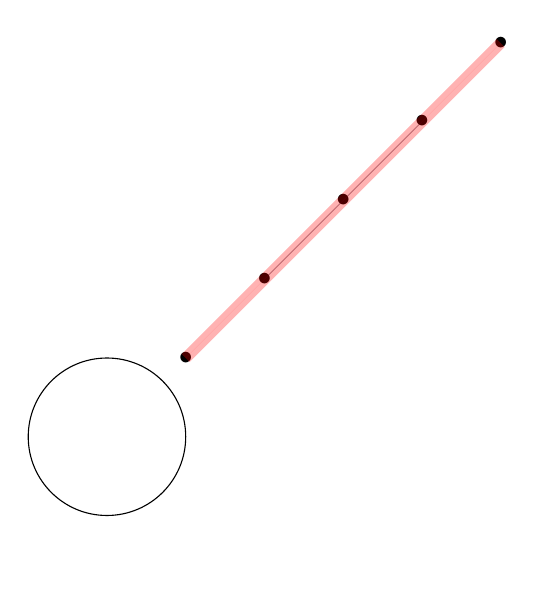
\begin{tikzpicture}
            \draw[fill=none](0,0) circle (1.0) node [black,yshift=-1.5cm]{};
            % Sample
            \coordinate (X1) at (\x1,\y1);
            \coordinate (X2) at (\x2,\y2); 
            \coordinate (X3) at (\x3,\y3); 
            \coordinate (X4) at (\x4,\y4); 
            \coordinate (X5) at (\x5,\y5); 
            \node[text=black] at (X1) {$\bullet$};
            \node[text=black] at (X2) {$\bullet$};
            \node[text=black] at (X3) {$\bullet$};
            \node[text=black] at (X4) {$\bullet$};
            \node[text=black] at (X5) {$\bullet$};
            \draw [draw=black, fill=blue, opacity=0.3]
        (X4) -- (X2) -- (X3) -- cycle;
        \draw [draw=red, line width=4pt, fill=red, opacity=0.3]
        (X1) -- (X5) -- cycle;
        \end{tikzpicture}
    }
    \subfloat{
        \begin{tikzpicture}
            \draw[fill=none](0,0) circle (1.0) node [black,yshift=-1.5cm]{};
            % Sample
            \coordinate (X1) at (\x1,\y1);
            \coordinate (X2) at (\x2,\y2); 
            \coordinate (X3) at (\x3,\y3); 
            \coordinate (X4) at (\x4,\y4); 
            \coordinate (X5) at (\x5,\y5); 
            \node[text=black] at (X1) {$\bullet$};
            \node[text=black] at (X2) {$\bullet$};
            \node[text=black] at (X3) {$\bullet$};
            \node[text=black] at (X4) {$\bullet$};
            \node[text=black] at (X5) {$\bullet$};
            \draw [draw=black, fill=blue, opacity=0.3]
        (X5) -- (X2) -- (X3) -- cycle;
        \draw [draw=red, line width=4pt, fill=red, opacity=0.3]
        (X4) -- (X1) -- cycle;
        \end{tikzpicture}
    }
    \subfloat{
        \begin{tikzpicture}
            \draw[fill=none](0,0) circle (1.0) node [black,yshift=-1.5cm]{};
            % Sample
            \coordinate (X1) at (\x1,\y1);
            \coordinate (X2) at (\x2,\y2); 
            \coordinate (X3) at (\x3,\y3); 
            \coordinate (X4) at (\x4,\y4); 
            \coordinate (X5) at (\x5,\y5); 
            \node[text=black] at (X1) {$\bullet$};
            \node[text=black] at (X2) {$\bullet$};
            \node[text=black] at (X3) {$\bullet$};
            \node[text=black] at (X4) {$\bullet$};
            \node[text=black] at (X5) {$\bullet$};
            \draw [draw=black, fill=blue, opacity=0.3]
        (X1) -- (X4) -- (X5) -- cycle;
        \draw [draw=red, line width=4pt, fill=red, opacity=0.3]
        (X2) -- (X3) -- cycle;
        \end{tikzpicture}
    }
    \subfloat{
        \begin{tikzpicture}
            \draw[fill=none](0,0) circle (1.0) node [black,yshift=-1.5cm]{};
            % Sample
            \coordinate (X1) at (\x1,\y1);
            \coordinate (X2) at (\x2,\y2); 
            \coordinate (X3) at (\x3,\y3); 
            \coordinate (X4) at (\x4,\y4); 
            \coordinate (X5) at (\x5,\y5); 
            \node[text=black] at (X1) {$\bullet$};
            \node[text=black] at (X2) {$\bullet$};
            \node[text=black] at (X3) {$\bullet$};
            \node[text=black] at (X4) {$\bullet$};
            \node[text=black] at (X5) {$\bullet$};
            \draw [draw=black, fill=blue, opacity=0.3]
        (X4) -- (X2) -- (X5) -- cycle;
        \draw [draw=red, line width=4pt, fill=red, opacity=0.3]
        (X1) -- (X3) -- cycle;
        \end{tikzpicture}
    }
    \subfloat{
        \begin{tikzpicture}
            \draw[fill=none](0,0) circle (1.0) node [black,yshift=-1.5cm]{};
            % Sample
            \coordinate (X1) at (\x1,\y1);
            \coordinate (X2) at (\x2,\y2); 
            \coordinate (X3) at (\x3,\y3); 
            \coordinate (X4) at (\x4,\y4); 
            \coordinate (X5) at (\x5,\y5); 
            \node[text=black] at (X1) {$\bullet$};
            \node[text=black] at (X2) {$\bullet$};
            \node[text=black] at (X3) {$\bullet$};
            \node[text=black] at (X4) {$\bullet$};
            \node[text=black] at (X5) {$\bullet$};
            \draw [draw=black, fill=blue, opacity=0.3]
        (X4) -- (X5) -- (X3) -- cycle;
        \draw [draw=red, line width=4pt, fill=red, opacity=0.3]
        (X1) -- (X2) -- cycle;
        \end{tikzpicture}
    }

    
    \caption{All 32 unique subsets of 5 points on $\S^1$}
\end{figure}

\newpage

\section{Vapnik–Chervonenkis inequality}

In the previous section we conclude that the uniform law of large numbers is satisfied for collections of sets with polynomial discrimination.

\begin{definition}
    Let $N_\AA (X_1,\ldots, X_n)$ be the number of different sets with the form $\{X_1,\ldots,X_n\}\cap A$ for $A \in \AA$
\[ N_\AA = \#\{\{X_1,\ldots,X_n\}\cap A \; ;\; A\in\AA\}.  \] 
The $n$-th shatter coefficient of the collection $\AA$ is the maximum of $N_\AA$ over all possible points in $S$:
\[ s(\AA, n) = \max_{X_1,\ldots, X_n \in S} N_\AA(X_1,\ldots, X_n) \leq 2^n. \]
Finally, the Vapnik–Chervonenkis dimension is defined as the largest integer $k$ for which $s(\AA, n) = 2^k$,
\[ V_A = \underset{k\in \N}{\text{argmax}} \{s(\AA, k) = 2^k\} = \underset{k\in \N}{\text{argmin}} \{s(\AA, k) < 2^k\} - 1. \]  
If $s(\AA, n) = 2^n$ for every $n\in \N$ or equivalently if $\AA$ doesn't have polynomial discrimination, we say that $V_A = \infty$.
\end{definition}

\begin{theorem}[Vapnik–Chervonenkis inequality]\label{vc:inequality}
 \[\P\{\|P_n-P\|_{\AA} > \varepsilon\} \leq s(\AA, n) \cdot e^{-n \varepsilon^2 / 32} \] 
\end{theorem}
\begin{proof}
    It might be anti-climatic to tell the reader that there's no work left in this proof. But let's recapitulate everything we've done so far:
    \begin{itemize}
        \item \textbf{First Symmetrization:} Using {lemma}~\ref{gc:l1} and Chebyshev's inequality we concluded that for an identical independent copy of the empirical measure $P_n'$ we have
        \[ \P\{\|P_n - P\|_\AA > \varepsilon\} \leq 2 \; \P\{\|P_n-P_n'\|_\AA > \tfrac{1}{2}\varepsilon\},\hspace*{1em}\text{for } n \geq \frac{8}{\varepsilon^2}.\] 
        \item \textbf{Second Symmetrization:} We build another distribution $P_n^\circ(A) = n^{-1}\sum \sigma_i \1_{X_i \in A} $ and concluded from {lemma}~\ref{gc:l2} equation~\ref{gc:2} that
        \[ \P\{\|P_n-P_n'\|_\AA > \tfrac{1}{2}\varepsilon\} \leq 2\; \P\{\|P_n^\circ\|_\AA > \tfrac{1}{4}\varepsilon\}   \]
        \item \textbf{Maximal Inequality:} This was the step in which we had to be most careful. In the rest of the steps it never really mattered if we worked with intervals or any other class of sets on any space. In this step the task is, for any given a sample $X_1, \ldots, X_n$, to find a sub-collection $\AA_n \subset \AA$ such that
        \[ \#\AA_n = \#\{\{X_1,\ldots,X_n\}\cap A \; ;\; A\in\AA\} = N_\AA(X_1,\ldots, X_n).\] 
        We proved the existence of this set in the previous theorem.
    \end{itemize}
\end{proof}

% Leer cap 4,12,13,18 Devroye
% chktex 17